% !TEX root =  master.tex
\chapter{Entwurf}\label{entwurf}
	\section[Design Entwurf]{Design Entwurf {\hfill \normalsize Milena Zahn}}	
		\begin{figure}[H]
			\centering 
			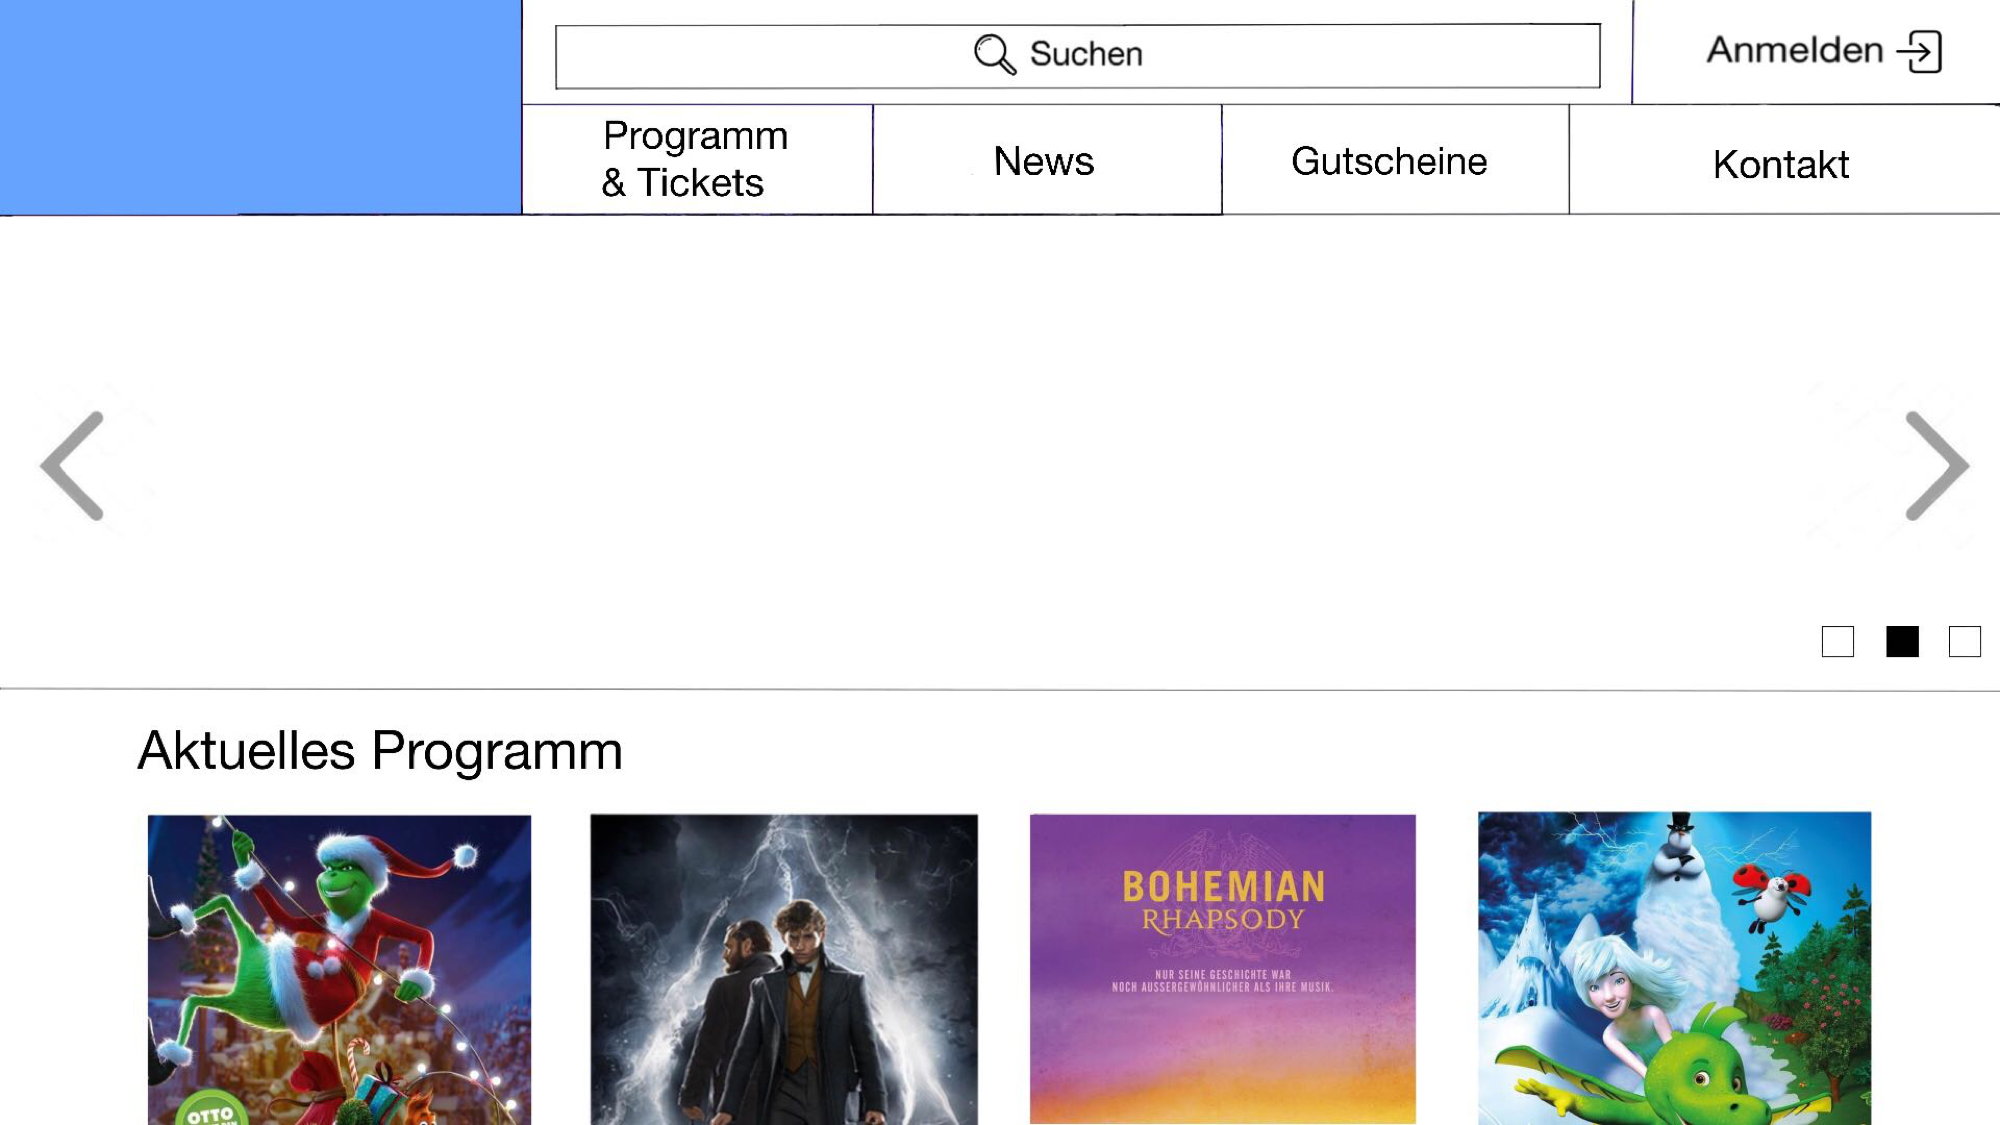
\includegraphics[width=14cm]{img/mockUp1.png}
			\captionsetup{format=hang}
			\caption[Mockup Startseite]{\label{fig:mockUpStartseite} Mockup Startseite }
		\end{figure}
		\begin{figure}[H]
			\centering 
			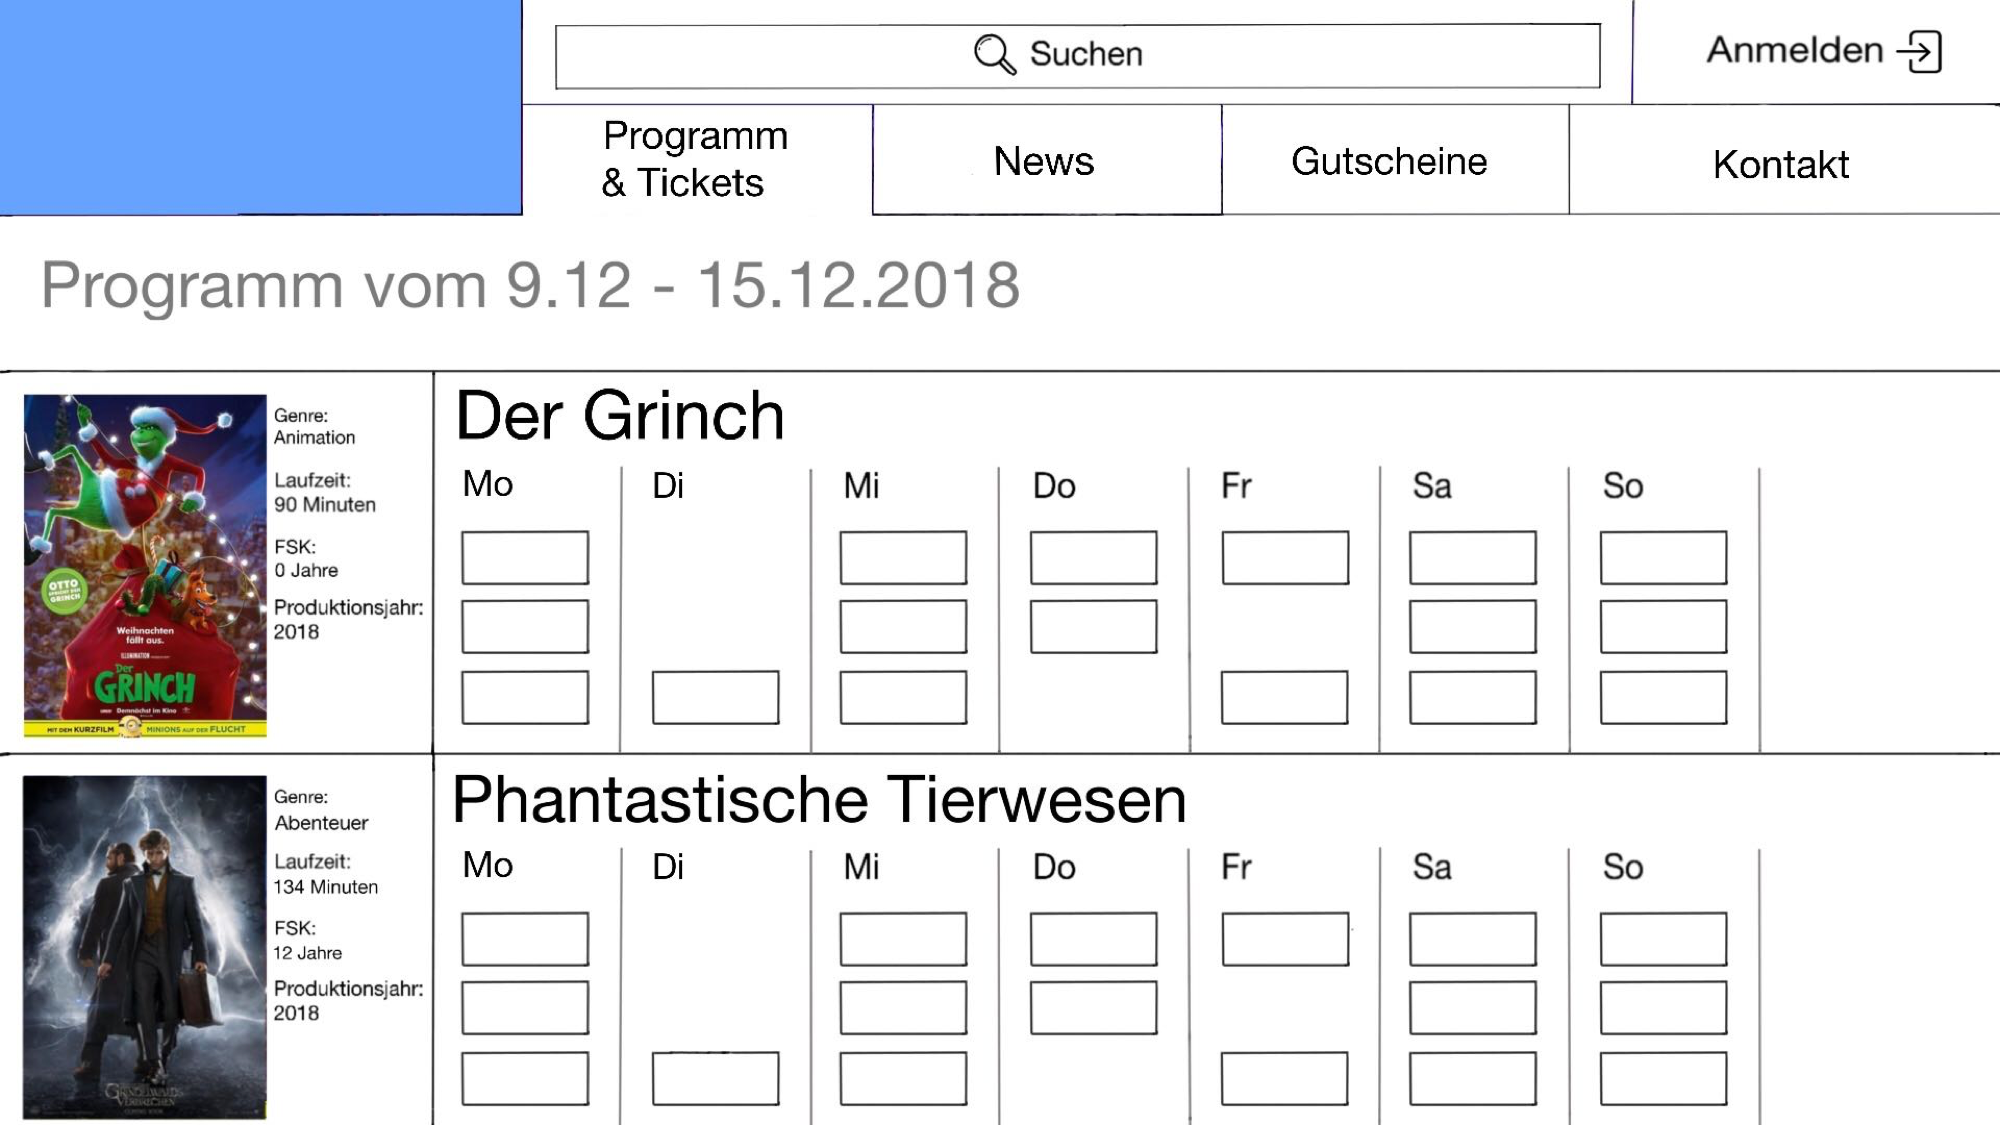
\includegraphics[width=14cm]{img/mockUp2.png}
			\captionsetup{format=hang}
			\caption[Mockup Programm]{\label{fig:mockUpProgramm} Mockup Programm }
		\end{figure}
		\begin{figure}[H]
			\centering 
			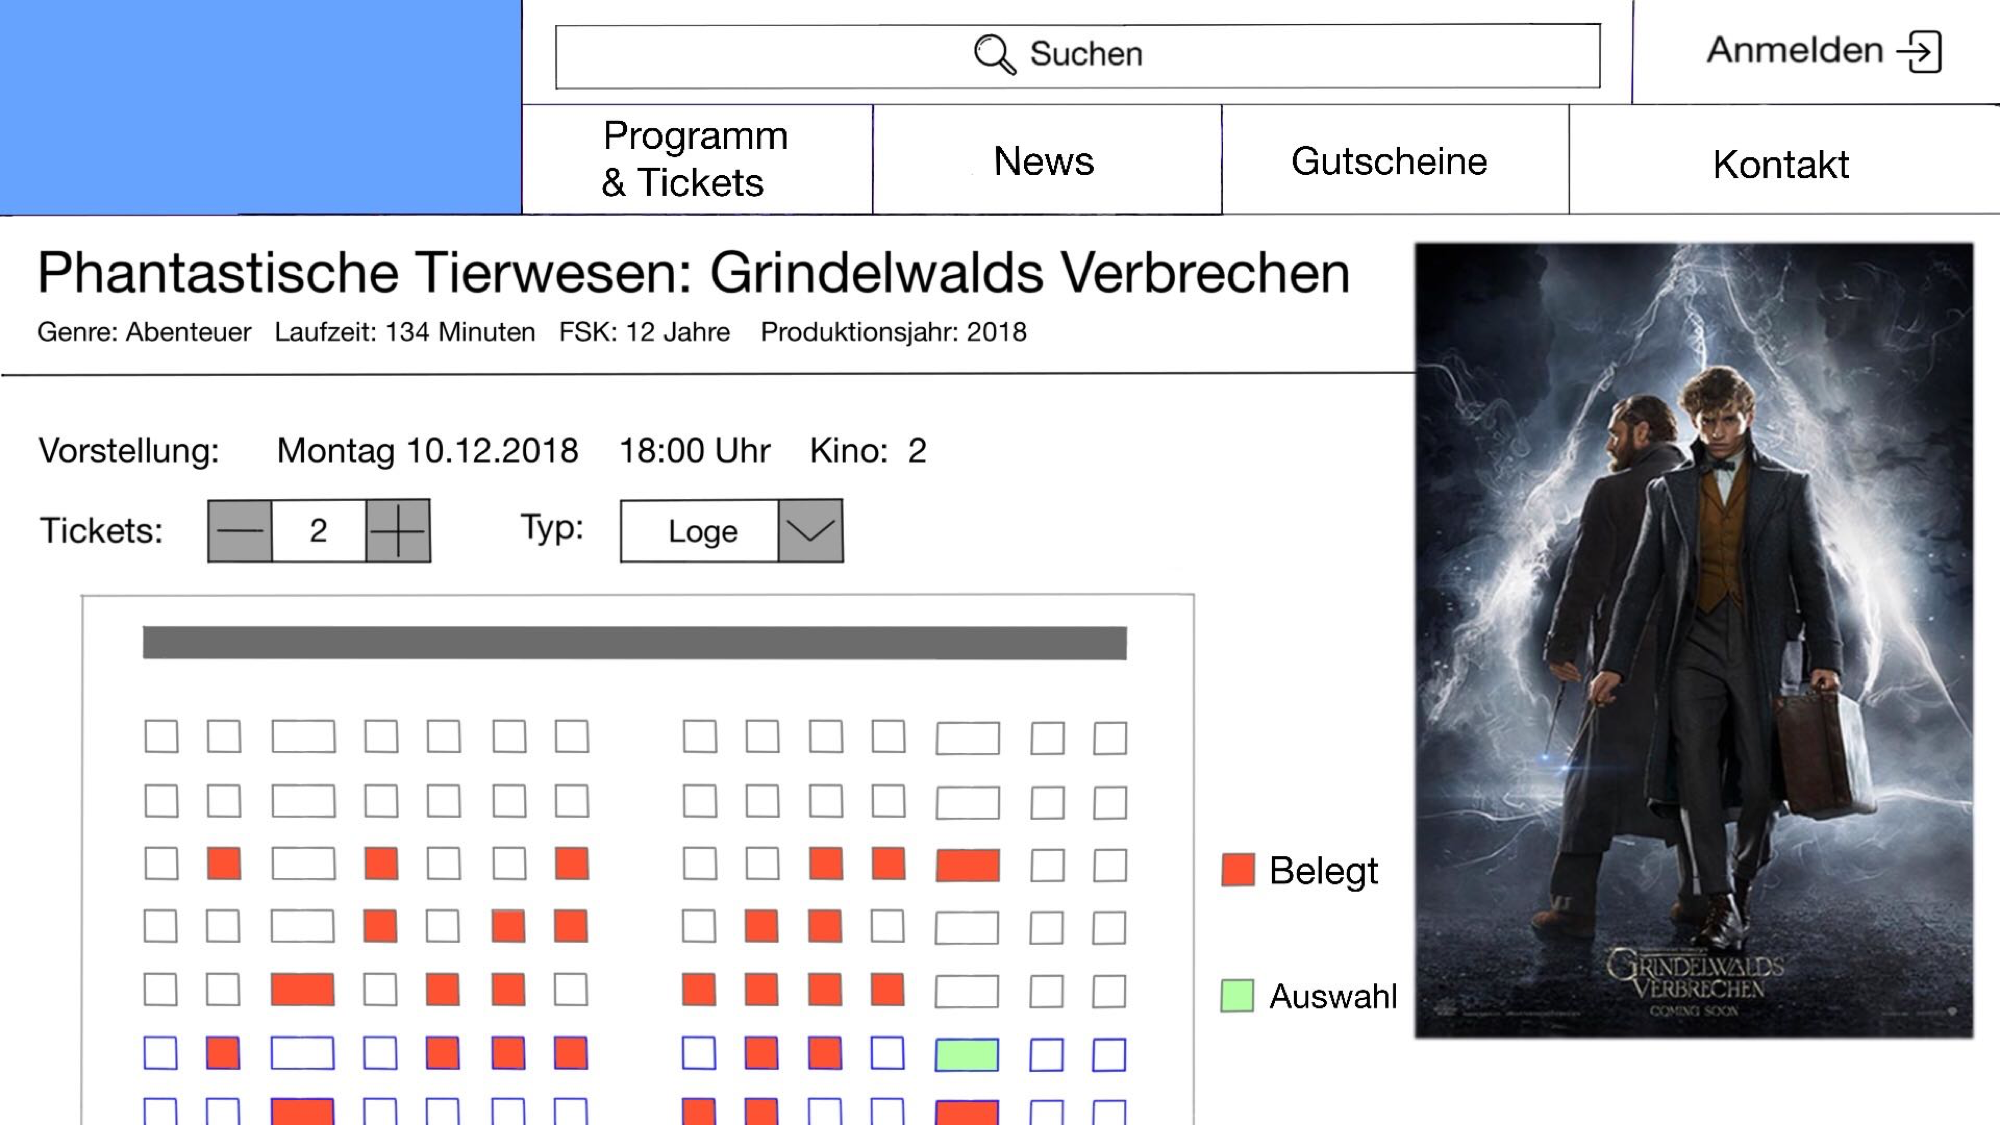
\includegraphics[width=14cm]{img/mockUp3.png}
			\captionsetup{format=hang}
			\caption[Mockup Sitzplan]{\label{fig:mockUpSitzplan} Mockup Sitzplan }
		\end{figure}
	
	\section[Technischer Entwurf]{Technischer Entwurf{\hfill \normalsize Felix Waage}} 	
	
		\section{Technischer Entwurf}
		Das \ac{ICS} ist ein komplexes Softwaresystem, welches aus verschiedenen Komponenten, Services und Schichten besteht. Aus diesem Grund war es bereits von Beginn an wichtig einen genauen Entwurf der späteren Softwarearchitektur zu entwickeln. Diese Vorgehensweise hat nicht nur den Vorteil, dass Zusammenhänge besser verstanden werden, sondern Probleme auch schneller zu finden und zu beheben sind. Darüber hinaus wird nur so eine effektive und gute Zusammenarbeit zwischen den Teammitgliedern ermöglicht und später die Wartung des gesamten Softwaresystem vereinfacht.
		Im weiteren Verlauf dieses Kapitel sollen die verschiedenen Schichten erläutert und deren Kommunikation untereinander beschrieben werden. Des Weiteren wird das Datenbankmodell definiert und näher auf die Architektur des Backends eingegangen.
		
		\subsection{Entwurfsprinzipien}
		Beim Entwurf eines Softwaresystem ist es besonders wichtig konsistent und gründlich zu arbeiten. Dies ist bedingt durch die Tatsache, dass immer mehrere Personen am \ac{ICS} arbeiten und den Entwurf verstehen müssen. Aus diesem Grund wurden vor Beginn der Entwicklung des Entwurfs einige Prinzipien festgelegt. Alle Prinzipien, welche folgend aufgelistet und erläutert werden, sollen unter anderem die Übersichtlichkeit, die Wartbarkeit und die Wiederverwendbarkeit des gesamten Projekts oder von Teilen davon ermöglichen.
		\begin{itemize}
			\item \textbf{Das Prinzip einer einzigen Verantwortung} -- Um die Komplexität und Organisation des Softwareprojekts beherschen zu können, wird das Projekt in verschiedene Module aufgeteilt. Dabei könne einzelene Module wieder aus anderen Modulen zusammen gesetzt sein. Es gilt so Komplexitäten aufzulösen. Jedes Modul übernimmt dabei genau eine Verantwortung und jede Verantwortung wir von genau einem Modul übernommen. Verantwortung ist in diesem Fall die Verpflichtung eine Anforderung umzusetzen. \autocite[Vgl.][]{Lahres.2015}
			\item \textbf{Trennung der Anliegen} -- Jedes Anliegen in einer Anwendung soll durch eigenes Modul realisiert werden. Ein mögliches Anliege wäre zum Beispiel die Transaktionssicherheit, welche unter anderem bei der Reservierung benötigt wird, jedoch auch bei weiteren Anforderung wiederverwendet werden können soll.\autocite[Vgl.][]{Lahres.2015} 
			\item \textbf{Wiederholungen vermeiden} -- Wenn gleiche Funktionalitäten in einem Softwaresystem mehrfach verwendet werden, sollte diese in ein Modul ausgelagert werden, um mögliche Redundanzen zu vermeiden. Dies könnte vor allem dann zum Problem führen, wenn im Code Fehler entdeckt wurden und dieser Fehler so an mehreren Stellen im Quelltext behoben werden muss. Dies stellt eine große Fehlerquelle dar und sollte somit vermieden werden.\autocite[Vgl.][]{Lahres.2015} 
			\item \textbf{Trennung der Schnittstelle von der Implementierung} -- Jedes Modul sollte nur von einer klar definierten Schnittstelle von einem anderen Modul abhängig sein. Dabei spielt die Implementierung der einzelnen Funktionalitäten keine Rolle. Der Quelltext der einzelnen Funktionalitäten soll demnach ausgetauscht werden können, ohne Änderungen an den Schnittstellenaufrufen vornehmen zu müssen. Dies macht das Softwaresystem verständlicher und einfacher zu warten.\autocite[Vgl.][]{Lahres.2015} 
			\item \textbf{Testbarkeit} -- Um direkt während der Entwicklung auf Fehler reagieren zu können ist es wichtig darauf zu achten, dass sich die einzelnen Module und Softwarekomponenten einzelnen Testen lassen. So werden neben der eigentlichen Funktionalität auch Unit-Test implementiert. Dies soll möglichst parallel zur Entwicklung der Funktionalität geschehen und muss beim Erstellen des Entwurfs beachtet werden.\autocite[Vgl.][]{Lahres.2015} 
		\end{itemize} 
		Wie in vermutlich jedem großen Softwareprojekt, kann es zu Sonderfällen kommen, wodurch nicht immer alle Prinzipien genau angewendet wurden. Im weiteren Verlauf dieses Kapitel wird an geeigneten Stellen noch einmal auf verschieden Prinzipien verwiesen, um deren Anwendung besser zu erläutern.
		\subsection{Schichtenmodell ICS}
		\begin{figure}[H]
			\centering 
			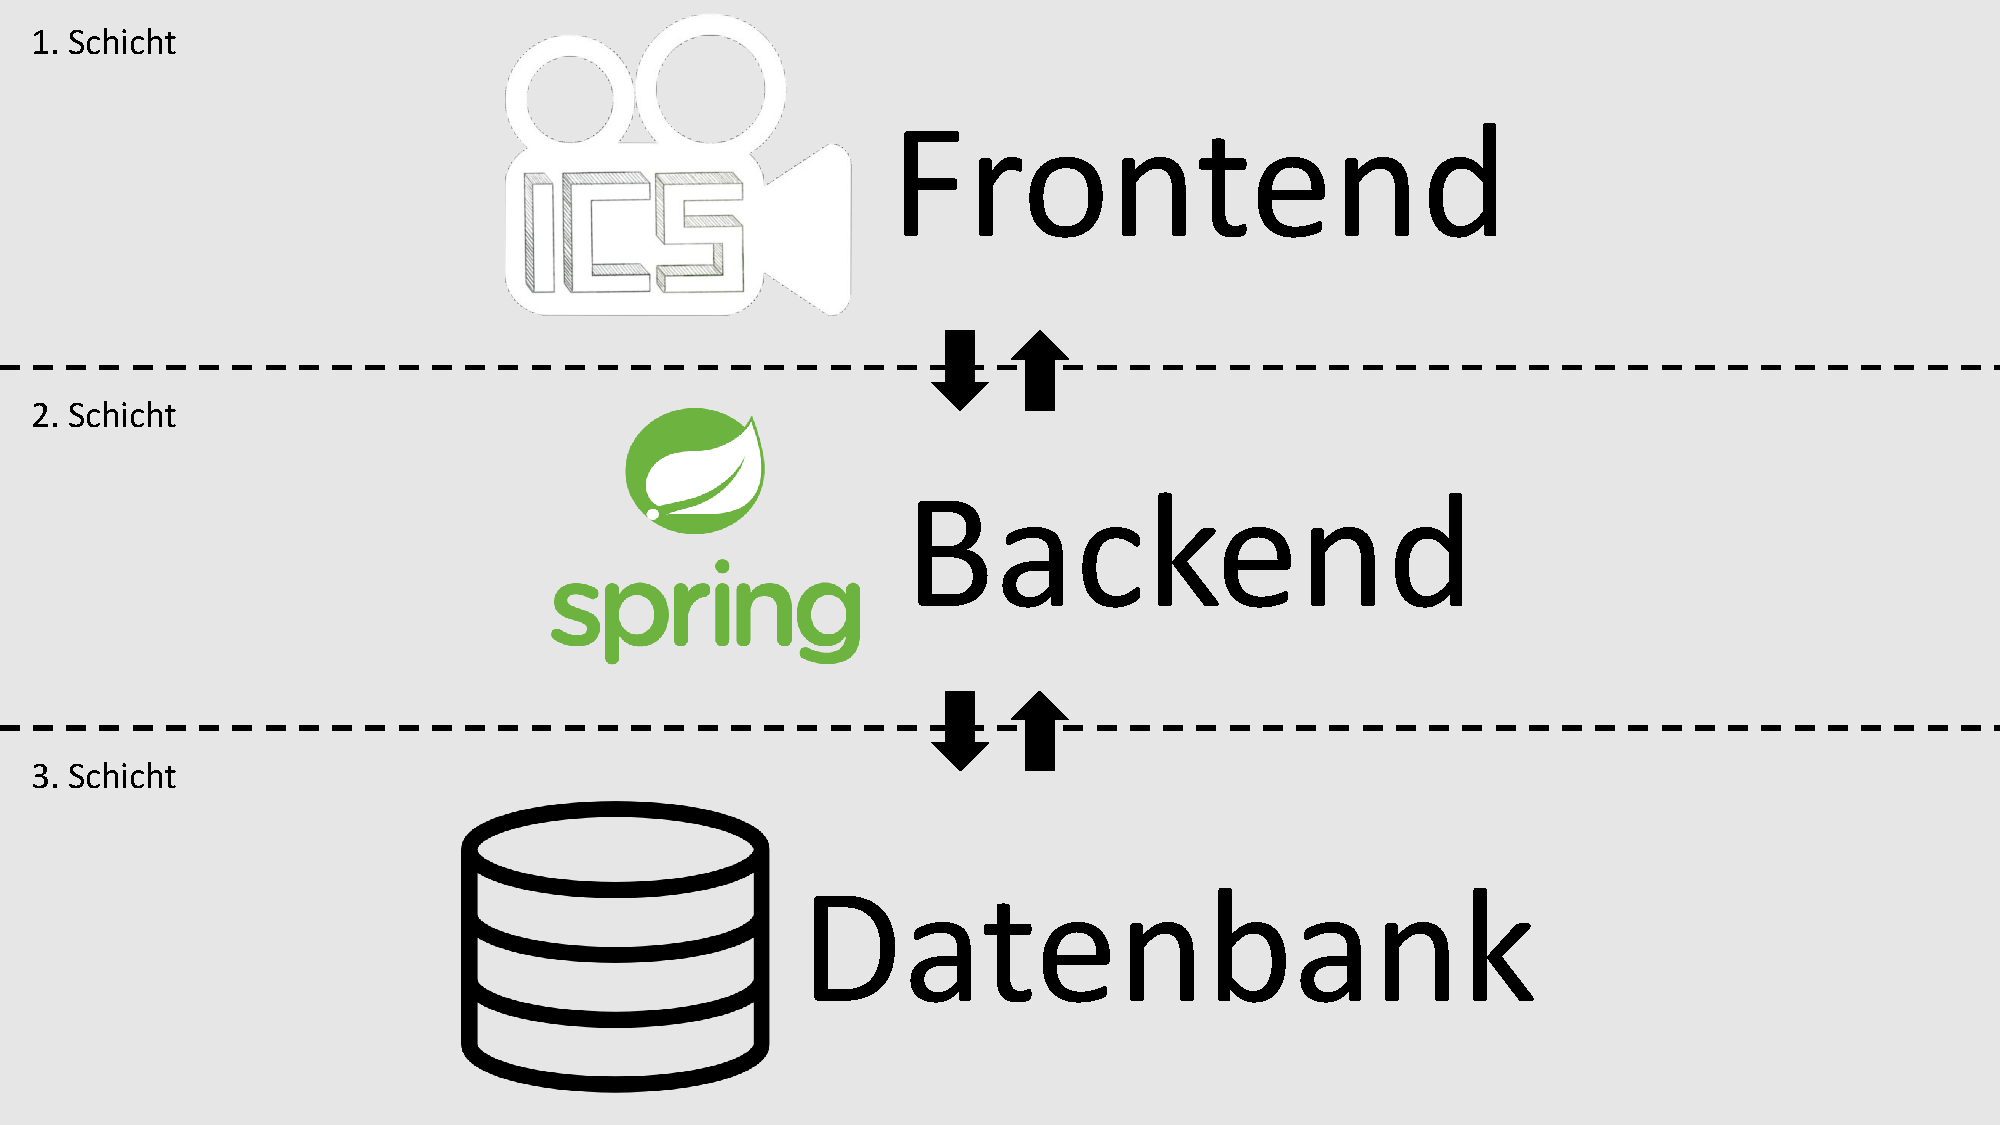
\includegraphics[width=14cm]{img/Schichtenmodell_ICS.pdf}
			\captionsetup{format=hang}
			\caption[Klassendiagramm]{\label{fig:Schichtenmodell} Schichtenmodell des ICS }
		\end{figure}
		Die Entwicklung des technischen Entwurfs für das \ac{ICS} wurde damit begonnen die notwendigen Schichten zu identifizieren und in Relation zueinander zu setzen. Es wurde beschlossen das Softwaresystem in drei Schichten aufzutrennen. 
		Die oberste Schicht ist das \glqq \textbf{Frontend}\grqq{}, welches die grafische Schnittstelle zum Benutzer darstellt. Über das Frontend kann der Benutzer zum Beispiel Filme suchen, Informationen zu Filmen einsehen und Tickets für eine Vorstellung reservieren. Diese Informationen erhält das Frontend durch HTTP-Request vom Backend.
		Im \glqq \textbf{Backend}\grqq{} ist die Fachlogik des Softwaresystem abgebildet, welche zum Beispiel zur Überprüfung der Korrektheit einer Reservierung benötigt wird. Darüber hinaus werden vom Backend die benötigten Restschnittstellen bereitgestellt und die Verbindung zur Datenbank organisiert. 
		Die \textbf{Dankbank} dient der Speicherung sämtlicher Daten und Informationen. Sie ist direkt mit dem Backend verbunden und nimmt Anfragen über SQL entgegen. 
		Für die Trennung des Softwaresystems in drei Schichten gibt es verschieden Gründe. Zum einen werden für die Implementierung des Frontends andere Technologien verwendet als für das Backend oder der Datenbank. Darüber hinaus verlangen die Anforderungen an das \ac{ICS} eine zentrale Datenhaltung, was sich am besten durch unterschiedliche Schichten realisieren lässt.
		\subsection{Statische Modelle}
		\begin{figure}[H]
			\centering 
			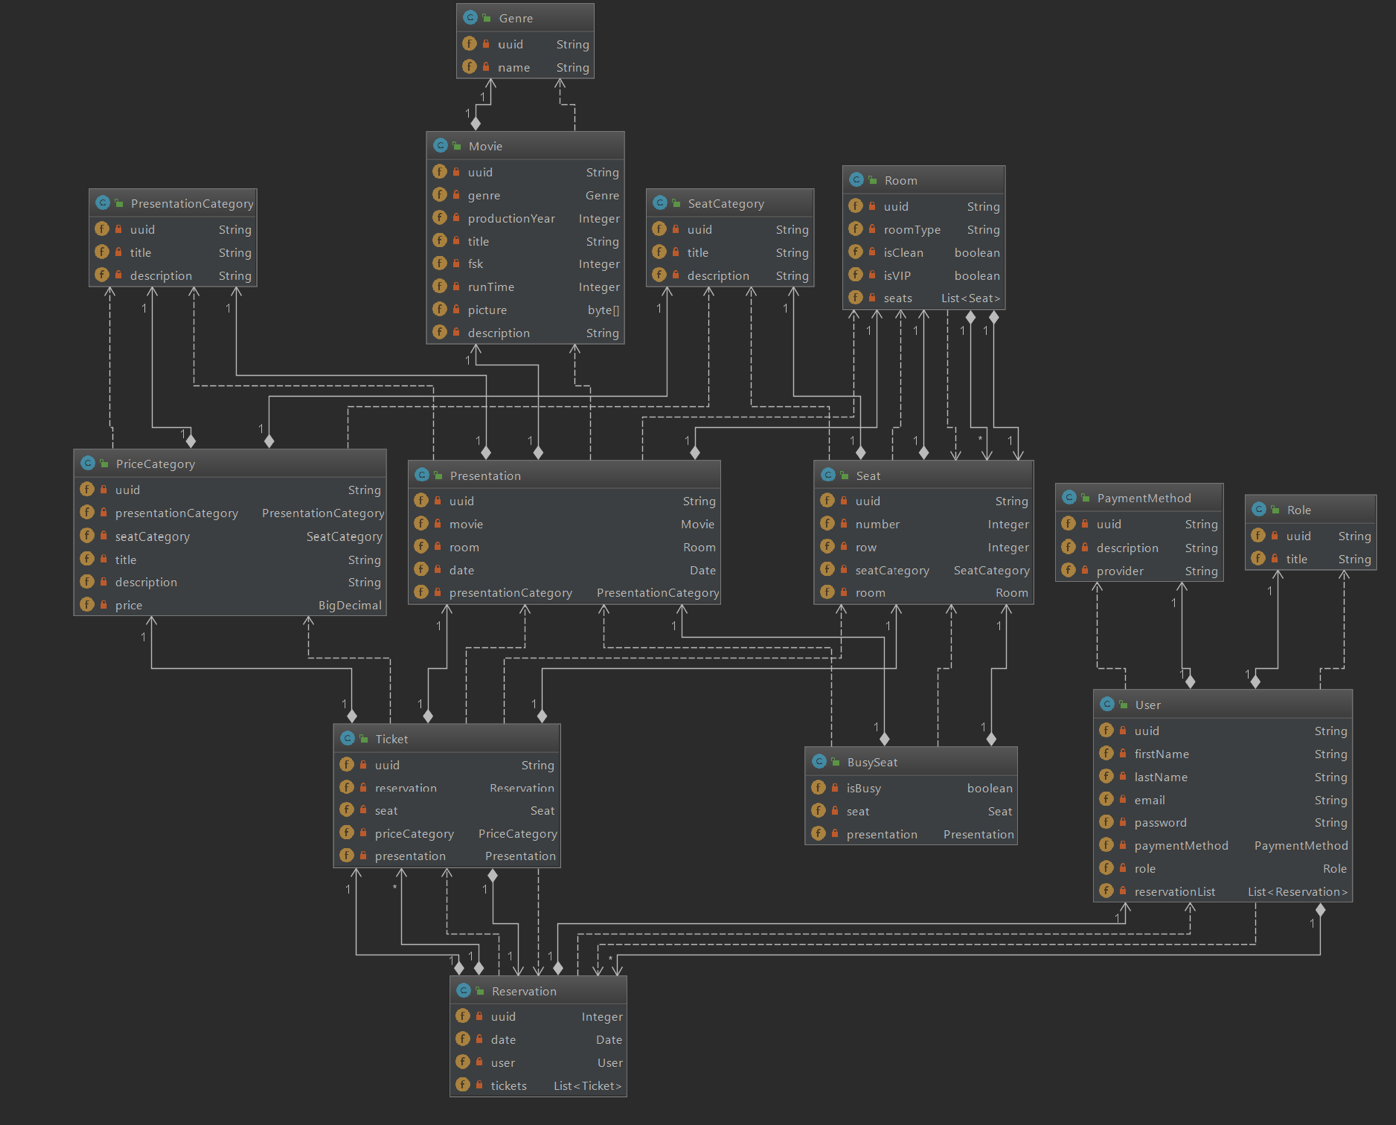
\includegraphics[width=14cm]{img/klassendiagramm.png}
			\captionsetup{format=hang}
			\caption[Klassendiagramm]{\label{fig:klassendiagramm} Klassendiagramm }
		\end{figure}
		
		\begin{figure}[H]
			\centering 
			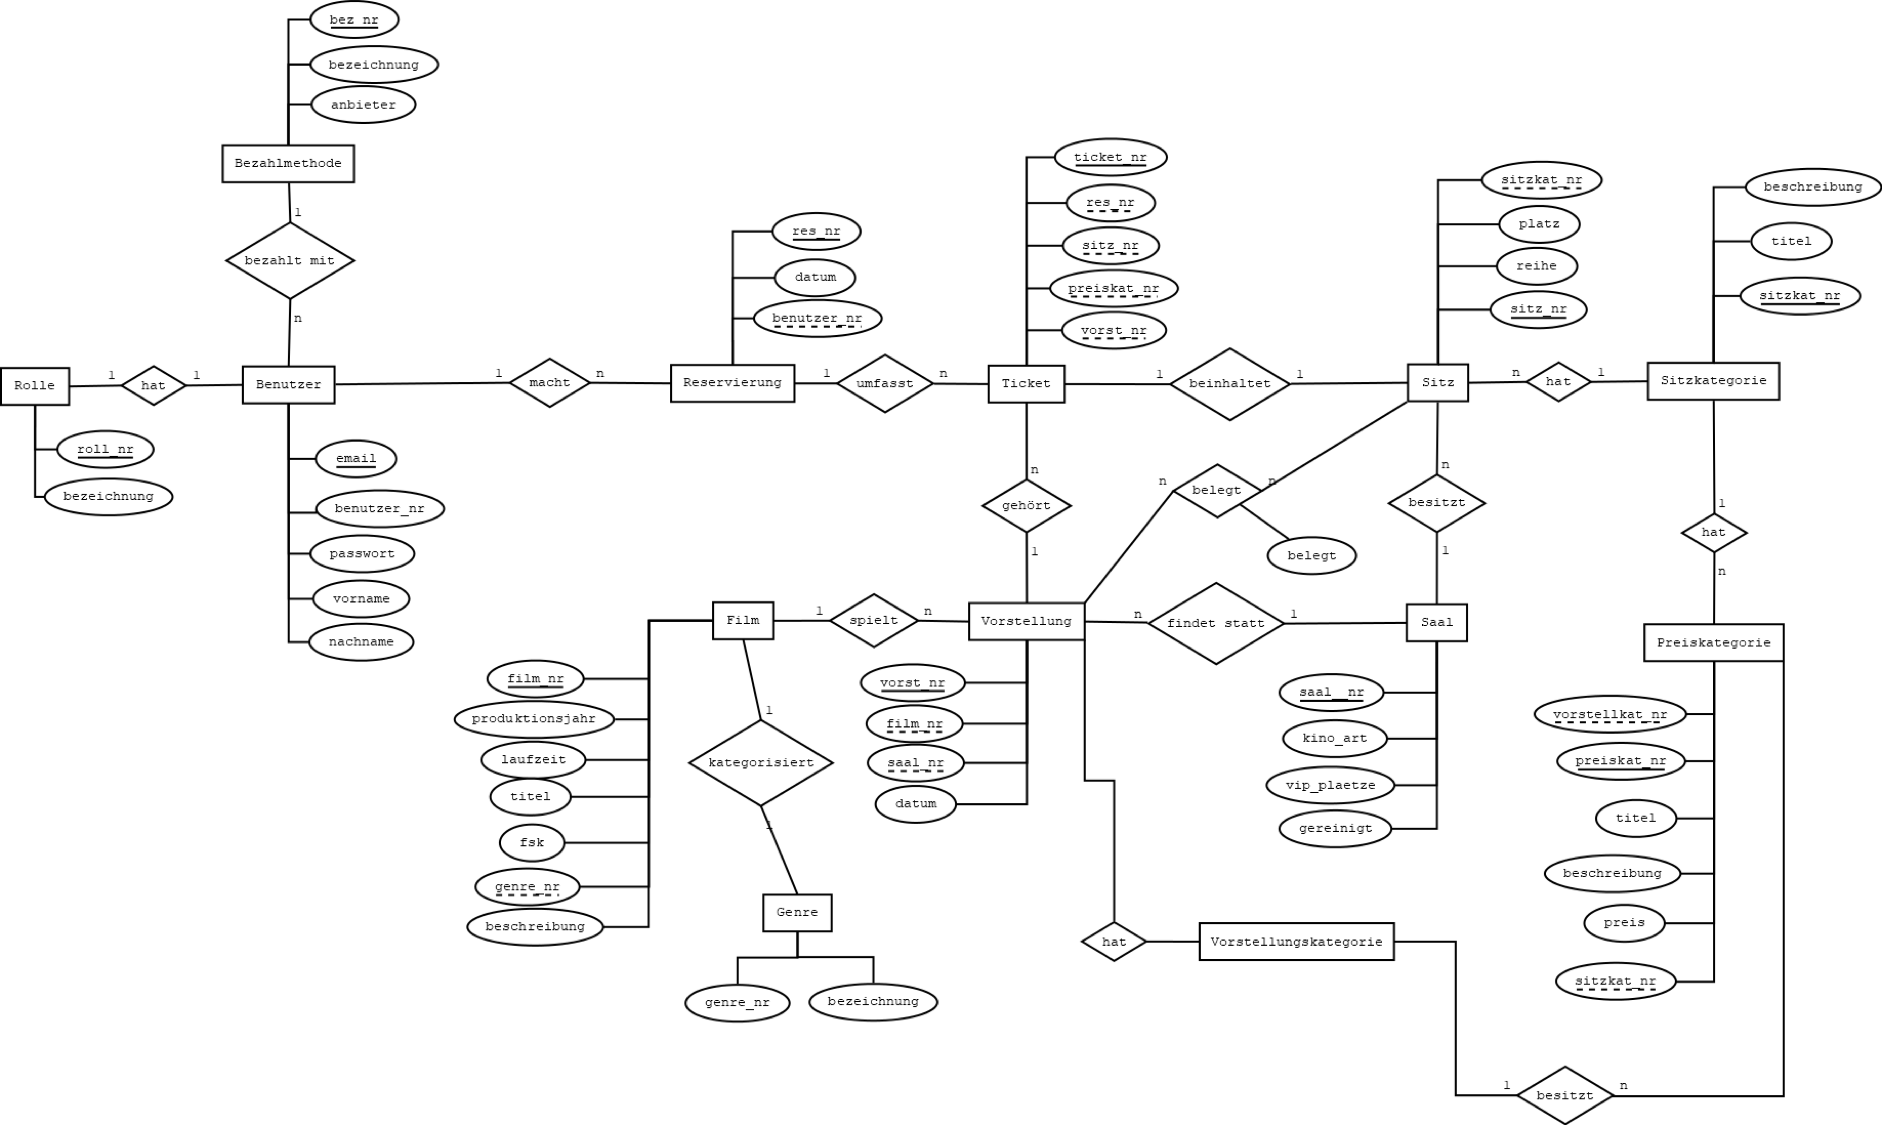
\includegraphics[width=15cm]{img/erModell.png}
			\captionsetup{format=hang}
			\caption[Entity Relationship Datenmodell]{\label{fig:erModell} Entity Relationship Datenmodell}
		\end{figure}
		
		\subsection{Dynamische Modelle}
		\begin{figure}[H]
			\centering 
			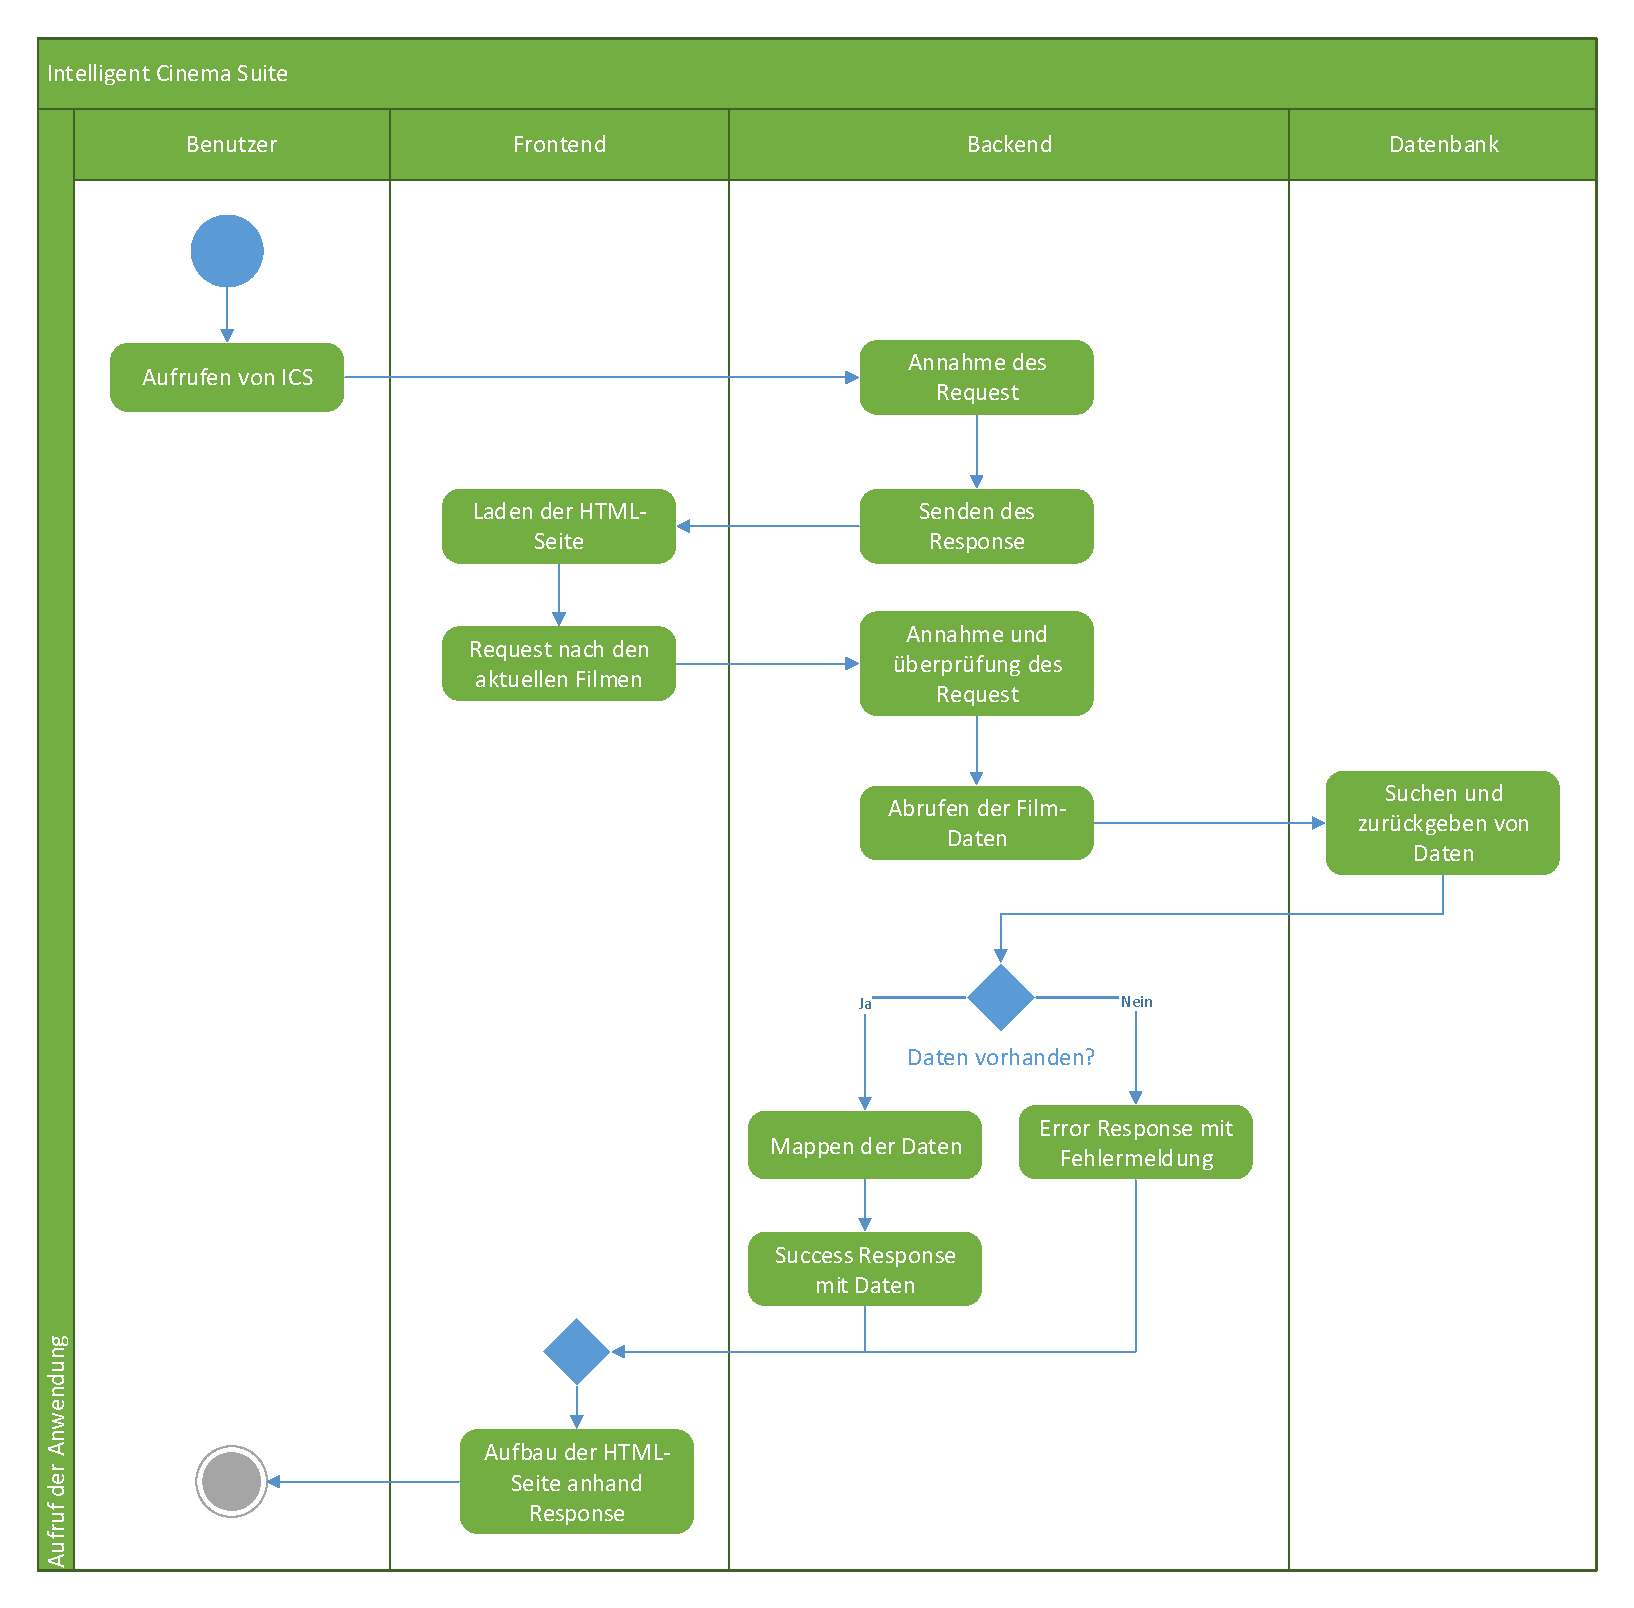
\includegraphics[width=15cm]{img/adSeitenaufruf.pdf}
			\captionsetup{format=hang}
			\caption[Aktivitätsdiagramm Seitenaufruf]{\label{fig:aktivitätSeitenaufruf} Aktivitätsdiagramm Seitenaufruf}
		\end{figure}
		
		%           \begin{figure}[H]
		%               \centering 
		%               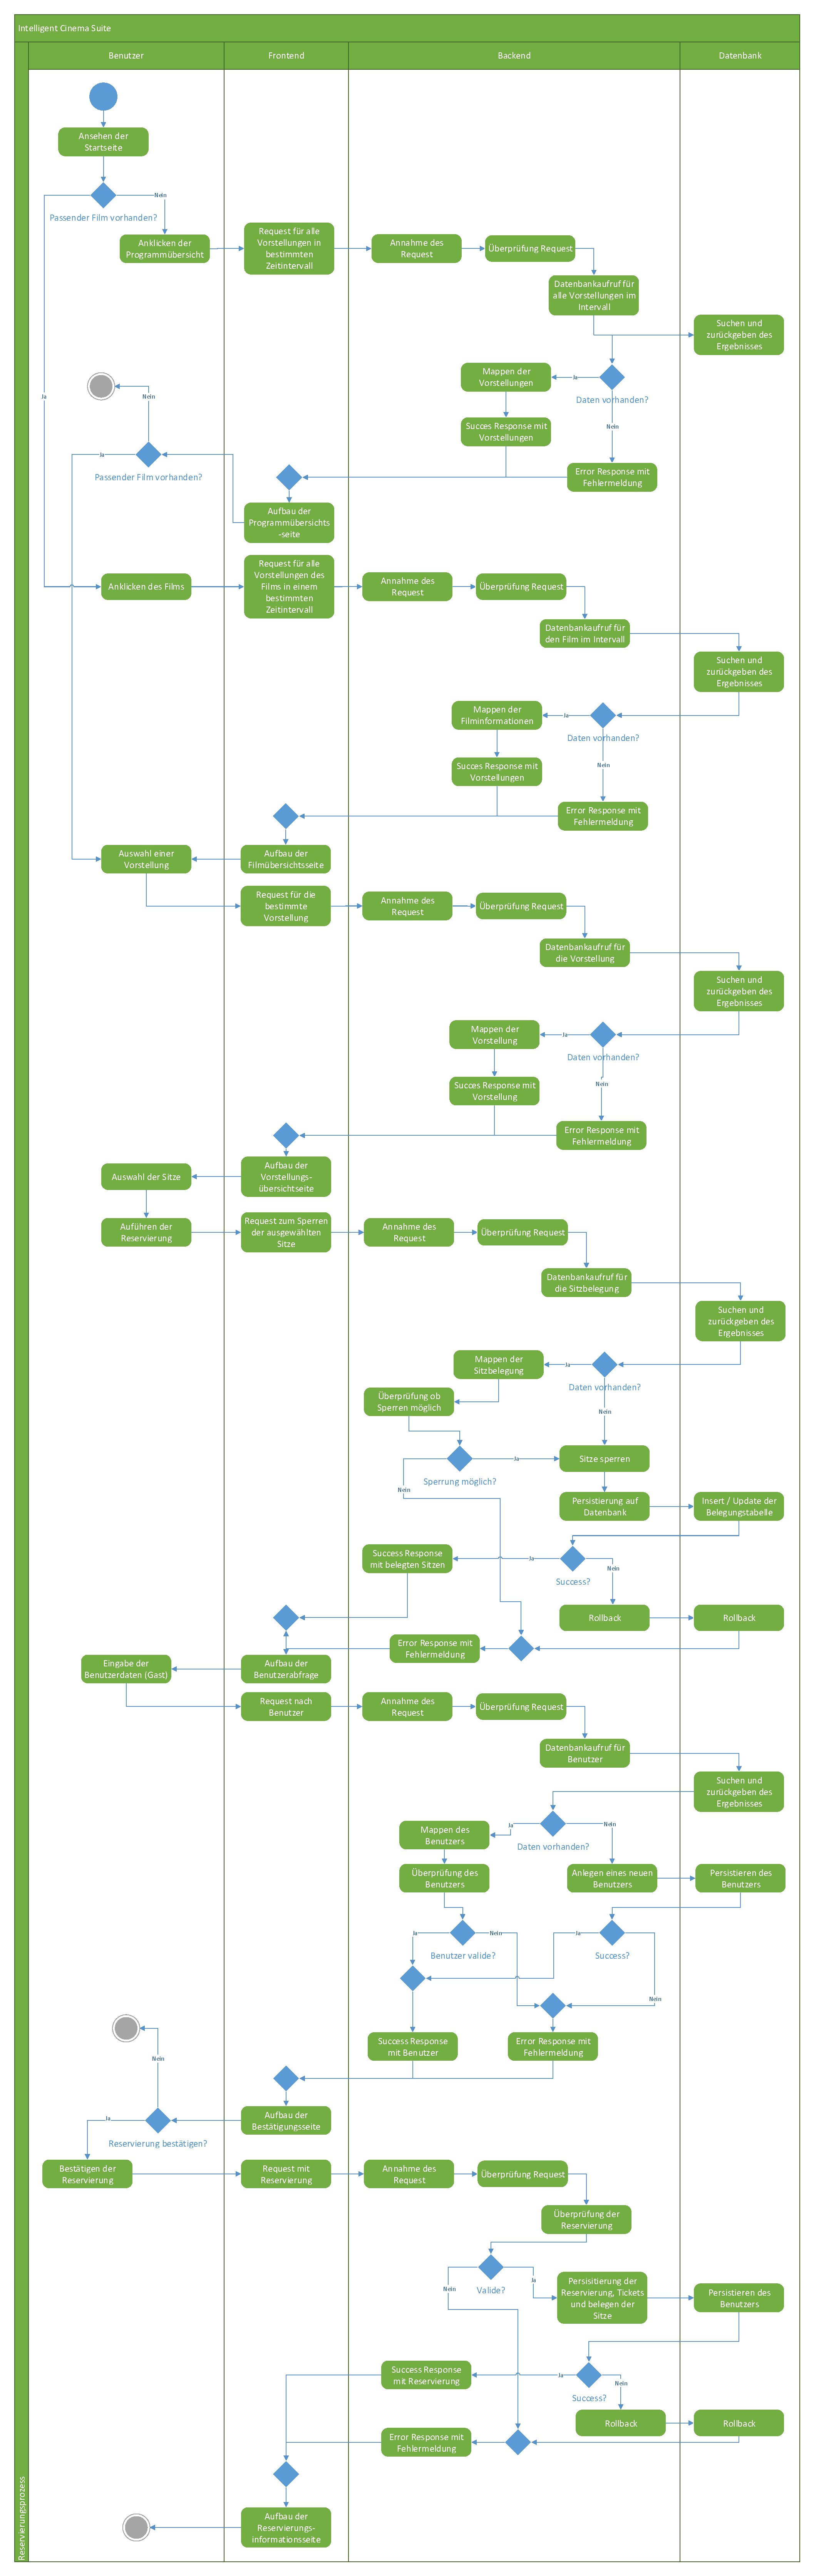
\includegraphics[width=14cm]{img/adReservierung.pdf}
		%               \captionsetup{format=hang}
		%               \caption[Aktivitätsdiagramm Seitenaufruf]{\label{fig:aktivitätSeitenaufruf} Aktivitätsdiagramm Reservierung}
		%           \end{figure}